\documentclass{article}

\usepackage[english]{babel}
\usepackage[utf8]{inputenc}
\usepackage{amsmath,amssymb}
\usepackage{parskip}
\usepackage{graphicx}


% Margins
\usepackage[top=2.5cm, left=3cm, right=3cm, bottom=4.0cm]{geometry}
% Colour table cells
\usepackage[table]{xcolor}


% Get larger line spacing in table
\newcommand{\tablespace}{\\[1.25mm]}
\newcommand\Tstrut{\rule{0pt}{2.6ex}}         % = `top' strut
\newcommand\tstrut{\rule{0pt}{2.0ex}}         % = `top' strut
\newcommand\Bstrut{\rule[-0.9ex]{0pt}{0pt}}   % = `bottom' strut

%%%%%%%%%%%%%%%%%
%     Title     %
%%%%%%%%%%%%%%%%%
\title{Camera Pose and 3D Points Estimation}
\author{Udit Singh Parihar \\ uditsinghparihar96@gmail.com}
\date{\today}

\begin{document}
\maketitle


\section{Problem Statement}
We are provided with images of checkerboard captured from 5 unknown camera locations. We are provided the 2D pixel locations of the captured images along with the point indicies
on the checkerboard. Checkerboard dimensions are provided in metric units. In the same environment, along checkerboard 3D point cloud is also captued. 3D point cloud has 10 3D 
points, whose positions are unknown. Our objective is to estimate the 5 camera pose and 10 3D points.

\subsection{Problem Setup}
Given camera matrix $K$:
% K matrix in math mode
\begin{align}
    K = \begin{bmatrix} f_x & 0 & c_x \\ 0 & f_y & c_y \\ 0 & 0 & 1 \end{bmatrix}
\end{align}

Here $f_x$ and $f_y$ are focal lengths equal to 200. And $c_x$ and $c_y$ are principal points equal to 0. 

Checkerboard dimensions are $1 \text{m} \times 1 \text{m}$. Checkerboard has 10 rows and 5 columns. Thus, we can calculate the 3D coordinates on the checkerboard, with the origin
in the top left corner as shown Figure \ref{fig:checkerboard}. Since all points lie on the same plane, Z coordinate is 0 for all points. These 3D coordinates on checkerboard along with the 2D pixel coordinates are used
to estimate the camera pose using Zhang method. All the camera poses and 3D point cloud location are calculated with respect to the world coordinate system, located at the origin of the checkerboard.

\begin{figure}[h!]
    \centering
    % Half column width image
    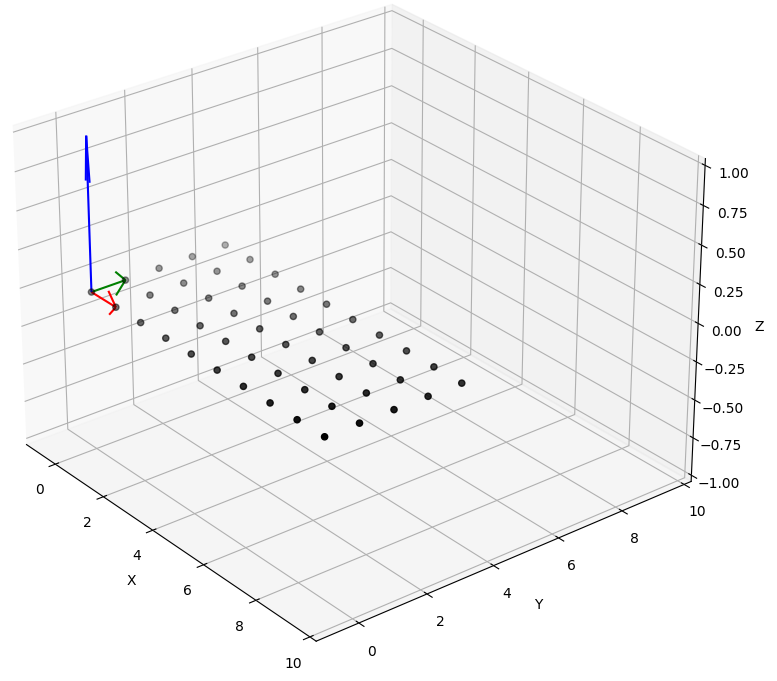
\includegraphics[width=0.8\textwidth]{images/checkerboard.png}
    \caption{Checkerboard with 3D coordinates in meters}
    \label{fig:checkerboard}
\end{figure}


\section{Methodology}
We first use provided checkerboard 2D pixels and corresponding 3D coordinates to calculate a homography matrix, $H$, using Zhang method. Then we decompose, $H$, into rotation, $R$, and translation, $t$, using SVD,
with a known camera matrix, $K$. The estimated camera poses, $R$ and $t$, are used to triangulate the 3D point cloud locations, using the provided 2D pixel coordinates. All the cameras are used to triangulate all the 3D 
points in the point clouds, as opposed to using only 2 cameras to triangulate a 3D point. Camera poses and 3D point cloud locations are obtained by solving linear equations of the form: $Ax = 0$.

In order to refine the estimated camera poses, $R$ and $t$, and point cloud 3D locations, we use the solution obtained from linear methods to initialize a bundle adjustment problem and the camera poses and point cloud
are jointly optimized.

\pagebreak
% Page 2

\subsection{Homography Estimation}
Camera projection equation can be written as:

\begin{equation}
    \begin{bmatrix}
    x_i \\ y_i \\ 1
    \end{bmatrix}_{3\times1} = \mathbf{K}_{3\times3}
    \begin{bmatrix}
    r_1 & r_2 & r_3 & t
    \end{bmatrix}_{3\times4}
    \begin{bmatrix}
    X_i \\ Y_i \\ Z_i \\1
    \end{bmatrix}_{4\times1}
\end{equation}

Now for planar checkerboard, $Z_i = 0$. So we can write the camera projection equation as:

\begin{equation}
    \begin{bmatrix}
    x_i \\ y_i \\ 1
    \end{bmatrix}_{3\times1} = \mathbf{K}_{3\times3}
    \begin{bmatrix}
    r_1 & r_2 & t
    \end{bmatrix}_{3\times3}
    \begin{bmatrix}
    X_i \\ Y_i \\ 1
    \end{bmatrix}_{3\times1}
\end{equation}

\begin{equation}
    \begin{bmatrix}
    x_i \\ y_i \\ 1
    \end{bmatrix}_{3\times1} = \mathbf{H}_{3\times3}
    \begin{bmatrix}
    X_i \\ Y_i \\ 1
    \end{bmatrix}_{3\times1}
\end{equation}

Let $P_i = \begin{bmatrix} X_i \\ Y_i \\ 1 \end{bmatrix}_{3 \times 1}$, then


\begin{equation}
    \begin{bmatrix}
    x_i \\ y_i \\ 1
    \end{bmatrix}_{3\times1} = \begin{bmatrix}H_{1}^{T} \\ H_{2}^{T} \\ H_{3}^{T}\end{bmatrix}_{3\times3}
    \mathbf{P_i}
\end{equation}

% Latex code for x_i = H_{1}^{T} P_i / H_{3}^{T} P_i  and y_i = H_{2}^{T} P_i / H_{3}^{T} P_i
\begin{equation}
    x_i = \frac{H_{1}^{T} P_i}{H_{3}^{T} P_i},\qquad
    y_i = \frac{H_{2}^{T} P_i}{H_{3}^{T} P_i}
\end{equation}

Taking all terms to the left side:

\begin{align}
    -H_{1}^T P_i + 0^T + x_i H_{3}^T P_i &= 0 \\
    0^T - H_2^T P_i + y_i H_{3}^T P_i &= 0
\end{align}

% Writing in a matrix form with variable in terms of H_1, H_2, H_3
\begin{equation}
    \begin{bmatrix}
    -P_{i}^T & 0^T & x_i P_{i}^T \\
    0^T_{1\times3} & (-P_i^T)_{1\times3} & (y_i P_{i}^T)_{1\times3}
    \end{bmatrix}_{2 \mathit{I}\times9}
    \begin{bmatrix}
    H_{1} \\ H_{2} \\ H_{3}
    \end{bmatrix}_{9\times1} = \begin{bmatrix}
    0 \\ 0
    \end{bmatrix}_{2 \mathit{I}\times1}
\end{equation}

Where $\mathit{I}$ is the number of 2D-3D correspondences from the checkerboard. In our case, $\mathit{I} = 50$. For each 2D-3D correspondence, we have 2 equations, so we have 100 equations in total. 
Let $\mathbf{M}$ be the matrix on the left side, then:

% M_{2(50) x 9} * [H_1 H_2 H_3]_{9 x 1} = 0_{2(50) x 1}
\begin{equation}
    \mathbf{M}_{100 \times 9} \begin{bmatrix} H_1 \\ H_2 \\ H_3 \end{bmatrix}_{9 \times 1} = \mathbf{0}_{100 \times 1}
\end{equation}

For obtaining the solution, $\vec{h}$, we can use SVD decomposition of $\mathbf{M}$:
\begin{align}
    \mathbf{M} &= \mathbf{U} \mathbf{\Sigma} \mathbf{V}^T \\
    \vec{h} &= V[:, -1] \\
    H &= \begin{bmatrix} h_1 & h_2 & h_3 \\ h_4 & h_5 & h_6 \\ h_7 & h_8 & h_9 \end{bmatrix}
\end{align}

Ensuring that the checkerboard lies in front of the camera, then $t_z$ or $H_{3,3}$ should be positive. Therefore, we can enforce this by multiplying $H$ with a sign of $H_{3,3}$.

\begin{equation}
    \mathbf{H} = sign(H_{3,3}) \mathbf{H}
\end{equation}

\subsection{Reprojection Error from Homography}
We can write the projected 2D points as:
% [x_i^{'} y_i^{'} 1]_{3 x 1} = H_{3 x 3} (P_i){3 x 1}
\begin{equation}
    \begin{bmatrix}
    x_i^{'} \\ y_i^{'} \\ 1
    \end{bmatrix}_{3 \times 1} = \mathbf{H}_{3 \times 3} \mathbf{P_i}_{3 \times 1}
\end{equation}

Reprojection error with respect to actual 2D pixels $x_i$ and $y_i$ is given by:

% summation from i = 1 to 50 || [xi' yi' 1] - [x_i y_i 1] ||_2

\begin{equation}
    error = \sum_{i=0}^{49} || \begin{bmatrix} x_i^{'} \\ y_i^{'} \\ 1 \end{bmatrix}_{3 \times 1} - \begin{bmatrix} x_i \\ y_i \\ 1 \end{bmatrix}_{3 \times 1} ||_2
\end{equation}

The above reprojection error for the homography for 5 camera poses is given in the Table \ref{tab:reprojection_error_homography}.

\begin{table}[h]
    \centering
    \begin{tabular}{|c|c|c|c|c|c|c|}
        \hline
        Camera Pose & Reprojection Error \\
        \hline
        0 & 1.160 \\
        1 & 1.144 \\
        2 & 1.167 \\
        3 & 1.146 \\
        4 & 1.268 \\
        Mean & 1.177 \\
        \hline
    \end{tabular}
    \caption{reprojection Error for Homography}
    \label{tab:reprojection_error_homography}
\end{table}

\subsection{Camera Pose Estimation}
We can obtain corresponding rotation matrix, $\mathbf{R}$, and translation vector, $\mathbf{t}$, from the homography matrix, $\mathbf{H}$, using the following equations:

% H = K[r1 r2|t]
\begin{align}
    \mathbf{H} &= \mathbf{K} \begin{bmatrix} \mathbf{r_1} & \mathbf{r_2} & | & \mathbf{t} \end{bmatrix} \\
    \mathbf{K}^{-1} \mathbf{H} &= \begin{bmatrix} \mathbf{r_1} & \mathbf{r_2} & | & \mathbf{t} \end{bmatrix}
\end{align}
    
Let, $\mathbf{K}^{-1} \mathbf{H} = \begin{bmatrix} h_1 & h_2 & h_3\end{bmatrix}$, then rotation matrix, $\mathbf{M}$ and translation vector, $\mathbf{t}$, can be obtained as:

% m1 = h1 / ||h1|| , m2 = h2 / ||h2||, m3 = m1 x m2
% M = [m1 m2 m3]
% t = h3 / ||h1||

\begin{align}
    \mathbf{M} &= \begin{bmatrix} \mathbf{m_1} & \mathbf{m_2} & \mathbf{m_3} \end{bmatrix} \\
    \mathbf{m_1} &= \frac{\mathbf{h_1}}{\|\mathbf{h_1}\|}  \\
    \mathbf{m_1} &= \frac{\mathbf{h_2}}{\|\mathbf{h_2}\|} \\
    \mathbf{m_3} &= \mathbf{m_1} \times \mathbf{m_2} \\
    \mathbf{t} &= \frac{\mathbf{h_3}}{\|\mathbf{h_1}\|}
\end{align}

The scaling factor of translation is the same scaling factor applied to the have unit norm of $\mathbf{m_1}$. 

Since the obtained $\mathbf{M}$ is not a rotation matrix, because we haven't enforced any orthogonality constraints between $\mathbf{m_1}$ and $\mathbf{m_2}$. 
And determinant of $\mathbf{M}$ is also not enforced to be 1. We can obtain a rotation matrix, $\mathbf{R} \in \mathrm{SO}(3)
$, by enforcing these constraints.


% R = argmin_{R in SO(3)} ||R - M||_F
% U S V^T = SVD(M)
% R = U [1 0 0; 0 1 0; 0 0 det(UV^T)] V^T

\begin{equation}
    \mathbf{R} = \arg\min_{\mathbf{R} \in \mathrm{SO}(3)} ||\mathbf{R} - \mathbf{M}||_F
\end{equation}
    
\begin{align}
    \mathbf{U}, \mathbf{S}, \mathbf{V}^T &= \mathrm{SVD}(\mathbf{M}) \\
    \mathbf{R} &= \mathbf{U} \begin{bmatrix} 1 & 0 & 0 \\ 0 & 1 & 0 \\ 0 & 0 & \mathrm{det}(\mathbf{U} \mathbf{V}^T) \end{bmatrix} \mathbf{V}^T
\end{align}

The final solution for 5 camera poses in world frame can be seen in Figure \ref{fig:env_cam_frame}.

\begin{figure}[h]
    \centering
    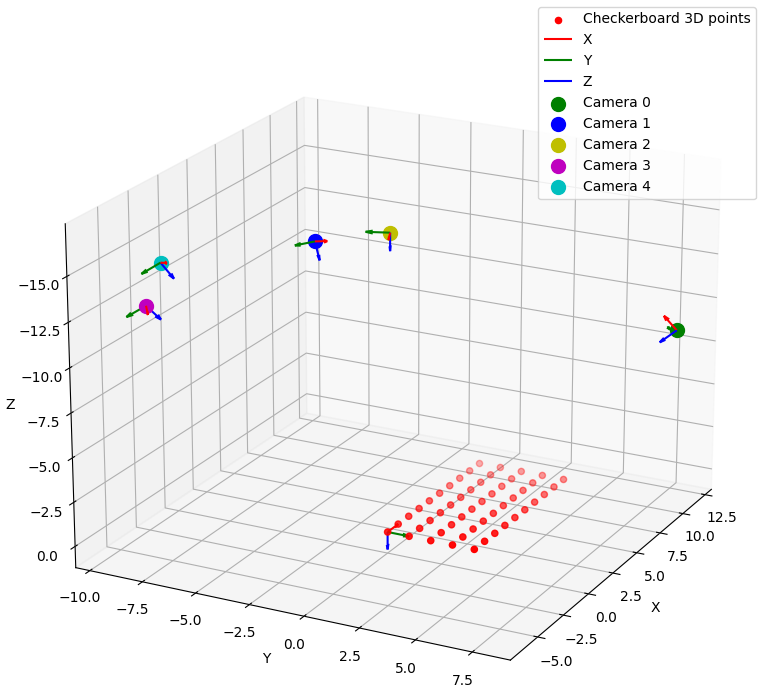
\includegraphics[width=0.8\textwidth]{images/env_cam_frame.png}
    \caption{Camera poses from Homogrpahy Decomposition of 2D-3D checkerboard correspondences}
    \label{fig:env_cam_frame}
\end{figure}



\subsection{Reprojection error from Rotation and Translation}
We can write the projected points $\begin{bmatrix} \mathbf{x_i}^{'} \mathbf{y_i}^{'} \end{bmatrix}^T$, in terms of given camera matrix, $\mathbf{K}$ and estimated rotation matrix, 
$\mathbf{R}$ and translation vector, $\mathbf{t}$, as:

\begin{equation}
    \begin{bmatrix} \mathbf{x_i}^{'} \\ \mathbf{y_i}^{'} \end{bmatrix} = \mathbf{K} \begin{bmatrix} \mathbf{R} & \mathbf{t} \end{bmatrix} \begin{bmatrix} \mathbf{X_i} \\ \mathbf{Y_i} \\ \mathbf{Z_i} \\ 1 \end{bmatrix}
\end{equation}

Here, $\mathbf{Z_i}=0$ for all the points on the checkerboard. Thus, reprojection error with respect to actual 2D pixels $x_i$ and $y_i$ is given by:

% summation from i = 1 to 50 || [xi' yi' 1] - [x_i y_i 1] ||_2

\begin{equation}
    error = \sum_{i=0}^{49} || \begin{bmatrix} x_i^{'} \\ y_i^{'} \\ 1 \end{bmatrix}_{3 \times 1} - \begin{bmatrix} x_i \\ y_i \\ 1 \end{bmatrix}_{3 \times 1} ||_2
\end{equation}

The reprojection error for the camera poses $\mathbf{R}$ and $\mathbf{t}$ for 5 camera poses is given in the Table \ref{tab:reprojection_error_r_t}.

\begin{table}[h]
    \centering
    \begin{tabular}{|c|c|c|c|c|c|c|}
        \hline
        Camera Pose & Reprojection Error \\
        \hline
        0 & 49.883 \\
        1 & 27.429 \\
        2 & 30.867 \\
        3 & 20.680 \\
        4 & 18.578 \\
        Mean & 29.487 \\
        \hline
    \end{tabular}
    \caption{Reprojection error from camera poses}
    \label{tab:reprojection_error_r_t}
\end{table}



\subsection{3D Point Cloud Estimation}
Now we know the camera poses in world frame, and we are given the 2D pixel coordinates of the points on the point cloud, $\vec{x_i} = \begin{bmatrix}
x_i \\ y_i
\end{bmatrix}$, we can estimate the 3D point cloud points, $\vec{X_i}$. Let our estimated, projection matrix, $\mathbf{P_i} = \mathbf{K} \begin{bmatrix} \mathbf{R_i} & \mathbf{t_i} \end{bmatrix}$. 
Then, a single point $\vec{X_1}$ can be triangulated from multiple views as:

\begin{equation}
    \begin{bmatrix} u_1 \\ v_1 \\ 1 \end{bmatrix} = \vec{x_1} = \mathbf{P_1} \vec{X_1}
\end{equation}

% u_1 = (P_1^1)^T X_1 / (P_1^3)^T X_1 and v_1 = (P_1^2)^T X_1 / (P_1^3)^T X_1
\begin{align}
    u_1 &= \frac{(\mathbf{P_1}^1)^T \vec{X_1}}{(\mathbf{P_1}^3)^T \vec{X_1}} \\
    v_1 &= \frac{(\mathbf{P_1}^2)^T \vec{X_1}}{(\mathbf{P_1}^3)^T \vec{X_1}}
\end{align}

% [[u_1 (P_3^1)^T - (P_1^1)^T]
% [v_1 (P_3^1)^T - (P_2^1)^T]
% [u_2 (P_3^2)^T - (P_1^2)^T]
% [v_2 (P_3^2)^T - (P_2^2)^T]
% [u_3 (P_3^3)^T - (P_1^3)^T]
% [v_3 (P_3^3)^T - (P_2^3)^T]
% [u_4 (P_3^4)^T - (P_1^4)^T]
% [v_4 (P_3^4)^T - (P_2^4)^T]] X_1 = 0

% \begin{equation}
%     \begin{bmatrix} u_1 (\mathbf{P_1}^3)^T - (\mathbf{P_1}^1)^T \\ v_1 (\mathbf{P_1}^3)^T - (\mathbf{P_1}^2)^T \\ u_2 (\mathbf{P_2}^3)^T - (\mathbf{P_2}^1)^T \\ v_2 (\mathbf{P_2}^3)^T - (\mathbf{P_2}^2)^T \\ u_3 (\mathbf{P_3}^3)^T - (\mathbf{P_3}^1)^T \\ v_3 (\mathbf{P_3}^3)^T - (\mathbf{P_3}^2)^T \\ u_4 (\mathbf{P_4}^3)^T - (\mathbf{P_4}^1)^T \\ v_4 (\mathbf{P_4}^3)^T - (\mathbf{P_4}^2)^T \end{bmatrix} \vec{X_1} = 0
% \end{equation}

\begin{equation*}
    \begin{bmatrix}
    u_1 (P_3^1)^T - (P_1^1)^T \\
    v_1 (P_3^1)^T - (P_2^1)^T \\
    u_2 (P_3^2)^T - (P_1^2)^T \\
    v_2 (P_3^2)^T - (P_2^2)^T \\
    u_3 (P_3^3)^T - (P_1^3)^T \\
    v_3 (P_3^3)^T - (P_2^3)^T \\
    u_4 (P_3^4)^T - (P_1^4)^T \\
    v_4 (P_3^4)^T - (P_2^4)^T \\
    u_5 (P_3^5)^T - (P_1^5)^T \\
    v_5 (P_3^5)^T - (P_2^5)^T \\
    \end{bmatrix}_{10 \times 4}
    {X_1} = 0
\end{equation*}

The solution to this system of equations, $A_{2 \times N} \vec{X_1} = 0$, is given by SVD decomposition of $A$:

% SVD(A) = UDV^T
% X_1 = V[:, -1]

\begin{align}
    \mathbf{U}, \mathbf{S}, \mathbf{V}^T &= \mathrm{SVD}(\mathbf{A}) \\
    \vec{X_1} &= \mathbf{V}[:, -1] \\
    \vec{X_1} &= \frac{\vec{X_1}}{\vec{X_1}[3]}
\end{align}

The final point cloud points, $\vec{X_i}$ along with camera poses and checkerboard points are shown in Figure \ref{fig:env_cam_frame_point_cloud}

\begin{figure}[h]
    \centering
    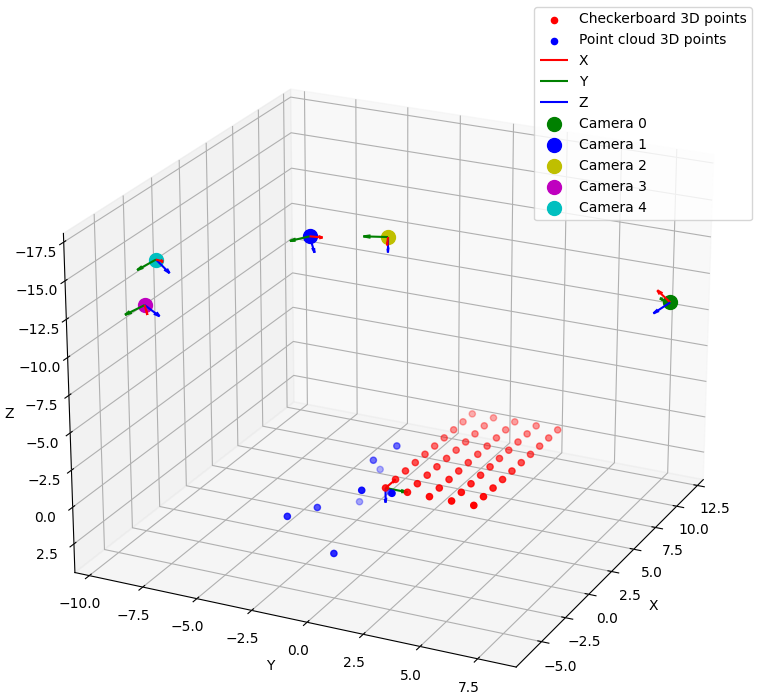
\includegraphics[width=0.7\textwidth]{images/env_cam_frame_point_cloud.png}
    \caption{Point cloud points, $\vec{X_i}$, camera poses, $\mathbf{P_i}$, and checkerboard points}
    \label{fig:env_cam_frame_point_cloud}
\end{figure}

Reprojection error for all the points in the point cloud for all the cameras is shown in Table \ref{tab:reprojection_error_point_cloud}.

\begin{table}[h]
    \centering
    \begin{tabular}{|c|c|c|c|c|c|c|}
        \hline
        Camera Pose & Reprojection Error \\
        \hline
        0 & 1.222 \\
        1 & 1.110 \\
        2 & 0.816 \\
        3 & 1.636 \\
        4 & 1.545 \\
        Mean & 1.266 \\
        \hline
    \end{tabular}
    \caption{Reprojection error of point cloud for all cameras}
    \label{tab:reprojection_error_point_cloud}
\end{table}


\subsection{Bundle Adjustment}
The estimated camera poses and point cloud points are used as initial estimates for bundle adjustment. Bundle adjustment is done to jointly optimized all the unknown parameters, i.e. camera poses and point cloud points. 
Camera projection equation for a 3D point $\vec{X_i}$, for camera $P_j$, observing pixel, $\vec{x_{ij}}$, is given by:

\begin{align}
    \begin{bmatrix} u_{ij} \\ v_{ij} \\ 1 \end{bmatrix} = \vec{x_{ij}} &= \mathbf{P_j} \vec{X_i} \\
    \begin{bmatrix} u_{ij} \\ v_{ij} \\ 1 \end{bmatrix} &= \begin{bmatrix}  {P_j^1}^T \\ {P_j^2}^T \\ {P_j^3}^T \end{bmatrix} \vec{X_i} \\
\end{align}

Reprojection error would be:

% L = summation j = 1 to 5 (summation i = 1 to 10 (u_{ij} - {P_j^1}^T X_i/({P_j^3}^T X_i))^2 + (v_{ij} - {P_j^2}^T X_i/({P_j^3}^T X_i))^2)

\begin{equation}
    L = \sum_{j=1}^{5} \sum_{i=1}^{10} \left( \left( u_{ij} - \frac{{P_j^1}^T X_i}{{P_j^3}^T X_i} \right)^2 + \left( v_{ij} - \frac{{P_j^2}^T X_i}{{P_j^3}^T X_i} \right)^2 \right)
\end{equation}

Our objective is:
% min(L) over X_i and P_j, where i = 1 to 10 and j = 1 to 5

\begin{equation}
    \min_{\vec{X_i}, \mathbf{P_j}} L
\end{equation}

Since, intrinsic matrix, $\mathbf{K}$ is known, we don't need to optimize over entire $\mathbf{P_j}$, but only over translation vector, $\vec{t_j}$ and rotation matrix, $\mathbf{R_j}$.
We can write a rotation matrix, $\mathbf{R}$ in axis angle form, $\vec{w}$ as:


% theta = ||\vec{w}||
% k = \vec{w}/ ||\vec{w}||
% K = [0 -k_3 k_2; k_3 0 -k_1; -k_2 k_1 0]

\begin{align}
    \theta &= ||\vec{w}|| \\
    k &= \frac{\vec{w}}{||\vec{w}||} \\
    K &= \begin{bmatrix} 0 & -k_3 & k_2 \\ k_3 & 0 & -k_1 \\ -k_2 & k_1 & 0 \end{bmatrix}
\end{align}

% R = I + sin(theta)K + (1 - cos(theta))K^2

\begin{equation}
    \mathbf{R} = \mathbf{I} + \sin(\theta) \mathbf{K} + (1 - \cos(\theta)) \mathbf{K}^2
\end{equation}

Thus for a single camera pose, we have 6 unknowns, i.e. 3 for translation vector, $\vec{t_j}$ and 3 for rotation vector, $\vec{w_j}$. For a single point in the point cloud, 
we have 3 unknowns, $X_i, Y_i, Z_i$. Thus, we have $6N + 3M$ unknowns, where $M$ is the number of points in the point cloud and $N$ is the number of cameras. 
The dimension of the residual vector is $2MN$. The Jacobian matrix is $2MN \times (6N + 3M)$. For our case $M = 10$ and $N = 5$, thus the dimension of the Jacobian matrix is $100 \times 60$.


\subsection{Bundle Adjustment Results}
We have used \textit{scipy.optimize.least\_squares} function to solve the bundle adjustment problem. It allows to provide the residual function, initial estimates and the sparsity pattern of the Jacobian matrix.
It calculates the Jacobian matrix and optimizes the non-linear and non-convex residual. The initial estimates for camera poses and point cloud points are obtained from the previous section.
Our initial and final root mean squared residual can be seen in table \ref{tab:bundle_adjustment_rmse}.

\begin{table}[h]
    \centering
    \begin{tabular}{|c|c|c|}
        \hline
        Initial RMSE & Final RMSE \\
        \hline
        1.0155 & 0.770 \\
        \hline
    \end{tabular}
    \caption{Root mean squared error of bundle adjustment}
    \label{tab:bundle_adjustment_rmse}
\end{table}

Since our initial estimates of camera pose and point cloud points are pretty accurate from Zhang method and multi view triangulation, therefore the bundle adjustment didn't improve the results much, and started 
pretty close to local minima. The bundle adjustment results can be seen in figure \ref{fig:bundle_adjustment_results}.

Values of optimized point cloud points with respect to world coordinate define at checkerboard corner is given in table \ref{tab:optimized_point_cloud_points}.

\begin{table}[h]
    \centering
    \begin{tabular}{|c|c|c|c|}
    \hline
    Point & X & Y & Z \\
    \hline
    1 & -1.862 & 1.164 & -1.030 \\
    2 & 1.919 & -1.140 & 0.137 \\
    3 & -3.185 & -3.029 & 0.981 \\
    4 & 0.859 & -0.180 & 0.830 \\
    5 & -1.914 & -0.188 & -0.836 \\
    6 & -1.723 & -2.336 & 1.003 \\
    7 & -2.938 & -1.022 & 2.984 \\
    8 & 1.237 & -0.040 & -2.126 \\
    9 & 0.891 & -1.618 & 1.831 \\
    10 & 0.641 & -0.841 & -1.222 \\
    \hline
    \end{tabular}
    \caption{Optimized point cloud points}
    \label{tab:optimized_point_cloud_points}
\end{table}


% page break
\pagebreak

\begin{figure}[h]
    \centering
    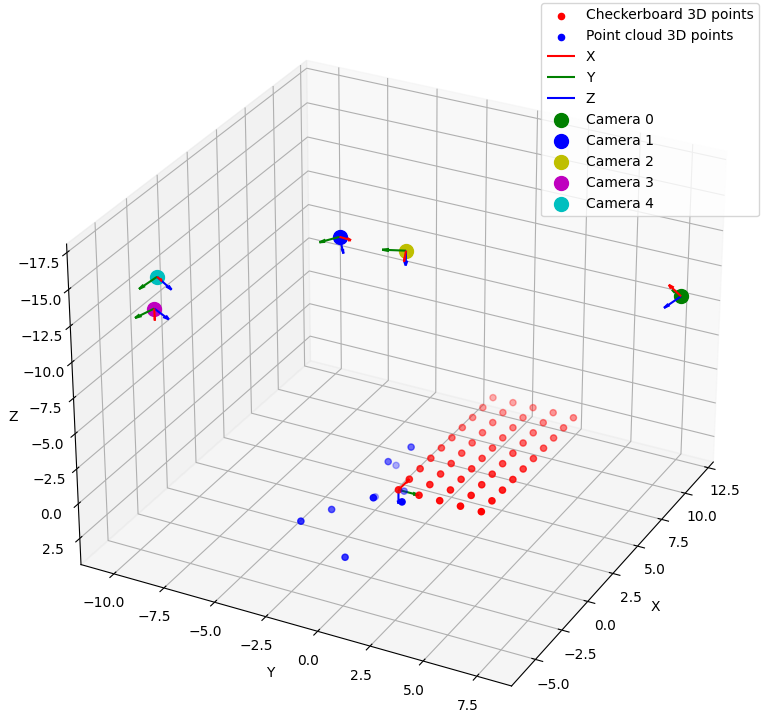
\includegraphics[width=0.8\textwidth]{images/bundle_adjustment_results.png}
    \caption{Bundle adjustment results}
    \label{fig:bundle_adjustment_results}
\end{figure}


\end{document}
